\documentclass[../../main.tex]{subfiles}
\begin{document}

\subsection*{8.7}
Una lamina conduttrice infinitamente lunga, di sezione rettangolare con lati $2a = 10\ cm$ e con $h=0.1\ cm$ è percorsa da una corrente di densità uniforme $j = 2\ \frac{A}{mm^2}$.
\\Calcolare il campo magnetico lungo l'asse y della lamina e il momento meccanico $\vec{M}$ che agisce su un piccolo ago magnetico di momento $m = 0.2\vec{u_y}\ Am^2$, posto a distanza $y_0 = 4\ cm$ dalla lamina.
\\Dimostrare che per $a \rightarrow \infty$ si ottengono i risultati dell'esercizio 8.8 e per $2a \ll y$ i risultati dell'esercizio 8.5.
\\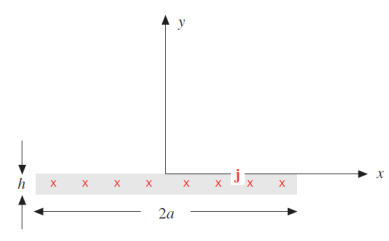
\includegraphics[scale=0.3]{e_8_7_0.png}
\\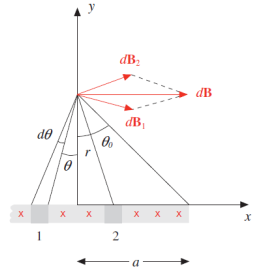
\includegraphics[scale=0.3]{e_8_7_1.png}
\subsubsection*{Formule utilizzate}
\subsubsection*{Soluzione punto a}
\subsubsection*{Soluzione punto b}
\newpage

\end{document}